\chapter*{Chapitre 2 : Méthodologie et Outils}
\addcontentsline{toc}{chapter}{Chapitre 2 : Méthodologie et Outils}

% ======= Introduction =======
\section{Introduction}
Ce chapitre décrit la méthodologie adoptée durant mon stage et les outils et technologies utilisés. L'objectif est de montrer comment l'organisation du travail et l'utilisation de technologies modernes ont facilité l'apprentissage, la collaboration et l'efficacité dans la réalisation des missions.\\

% ======= Méthodologie générale =======
\section{Méthodologie générale de travail}
\vskip.5cm
\begin{figure}[H]
    \centering
    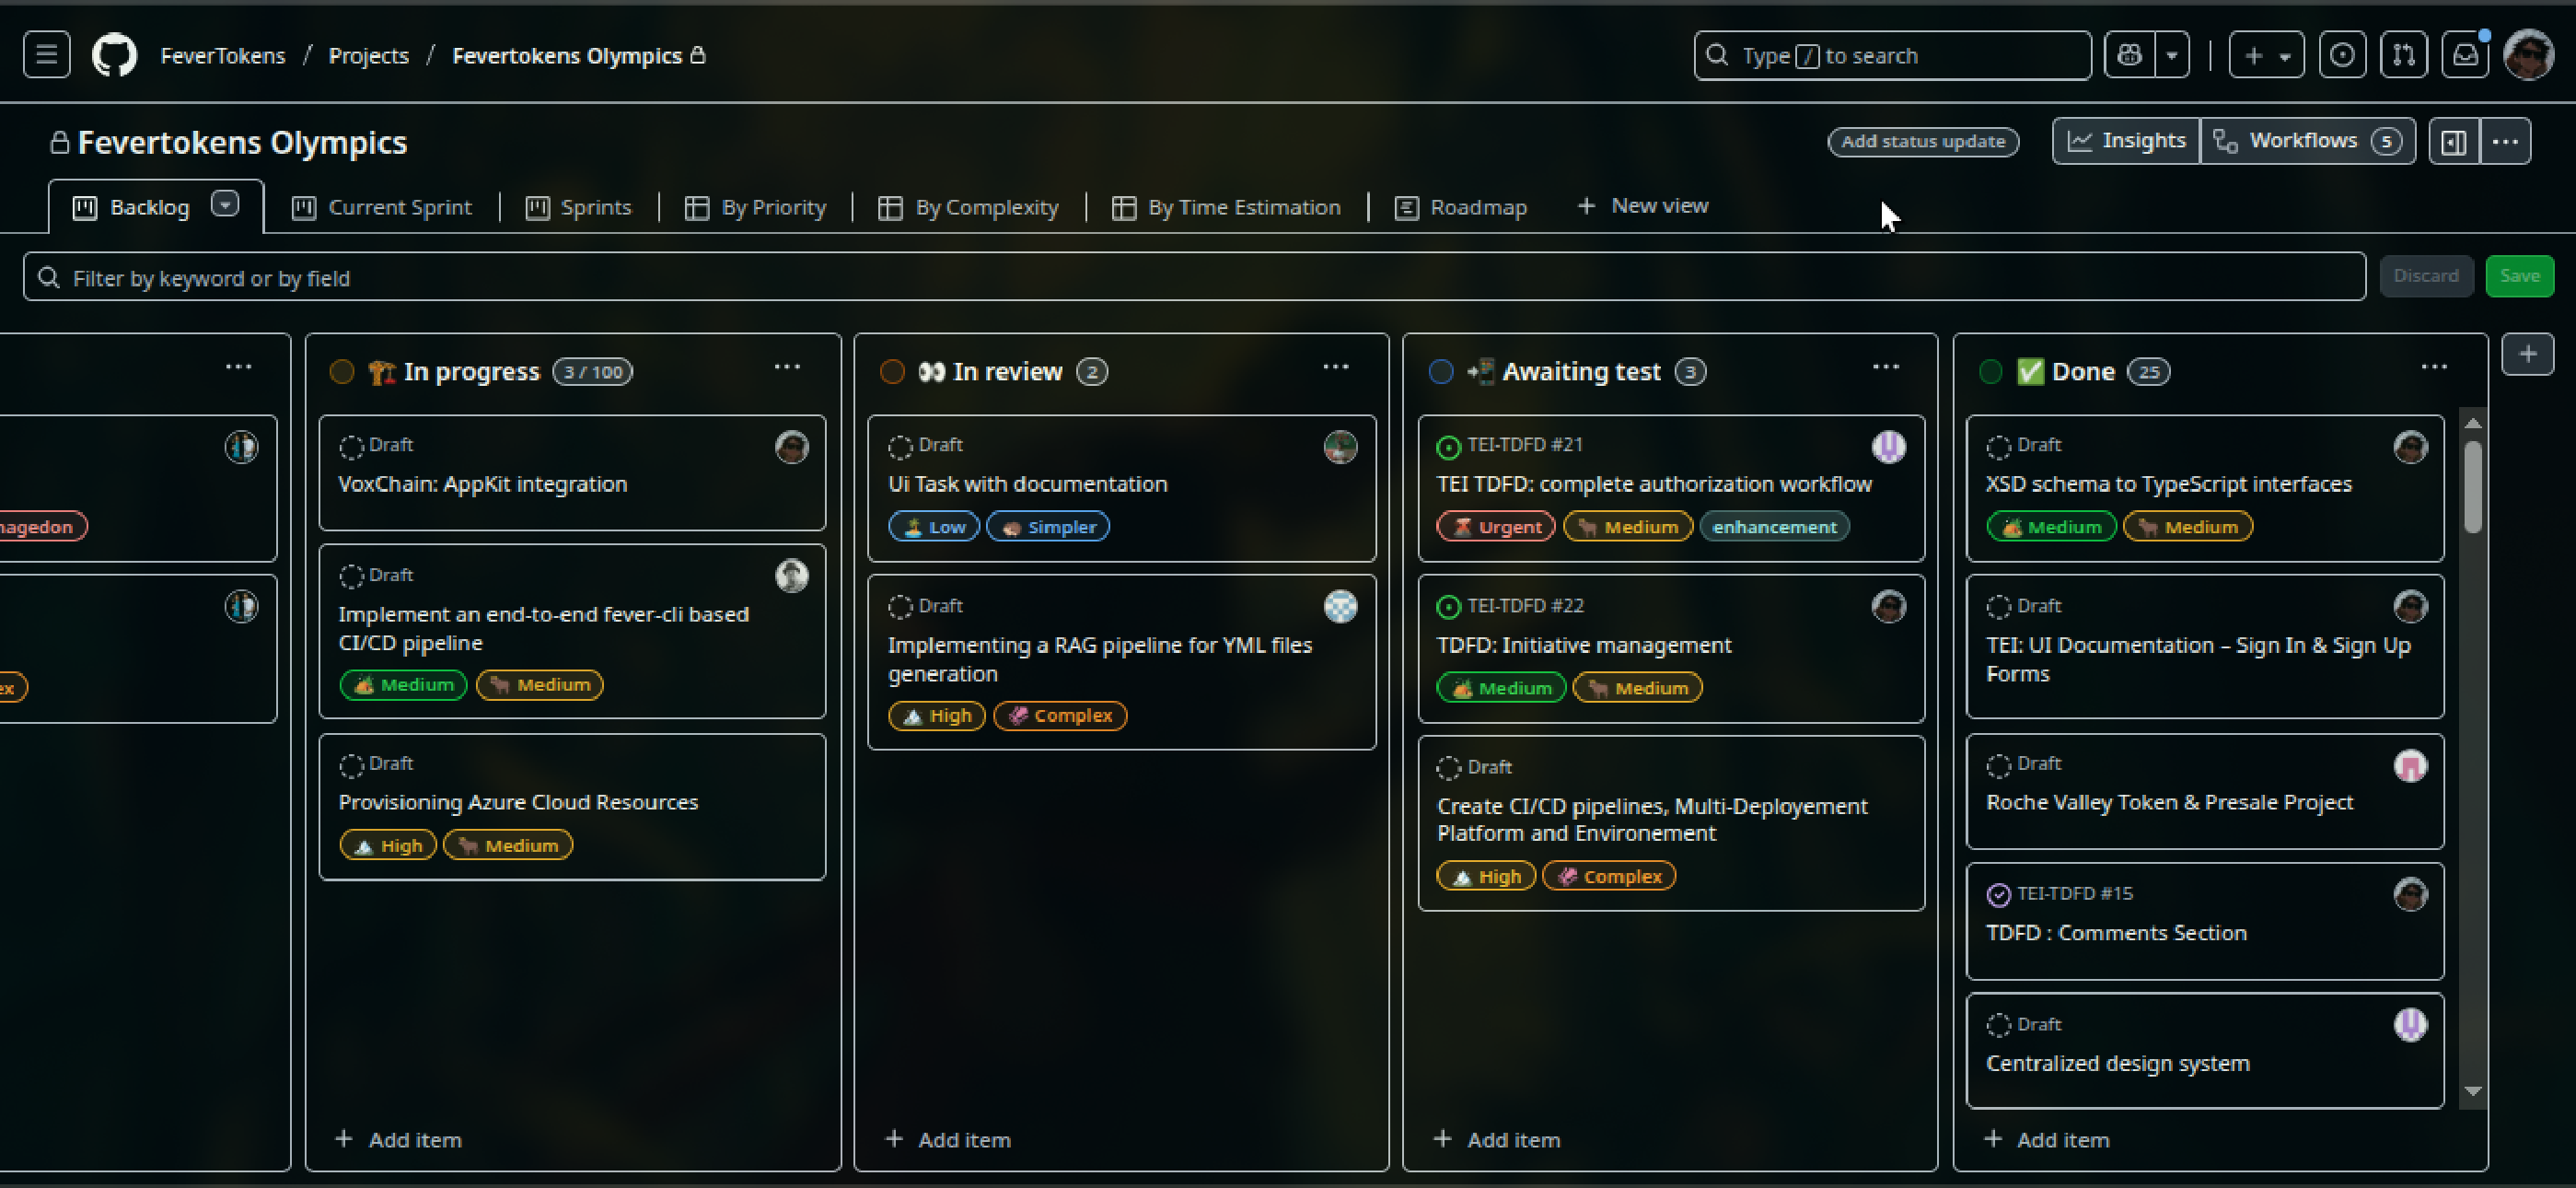
\includegraphics[width=0.7\textwidth]{figures/task-2.pdf}
    \caption{Plusieurs taches créées sur GitHub Projects}
    \label{fig:tache}
\end{figure}
\vskip.25cm
\begin{figure}[H]
    \centering
    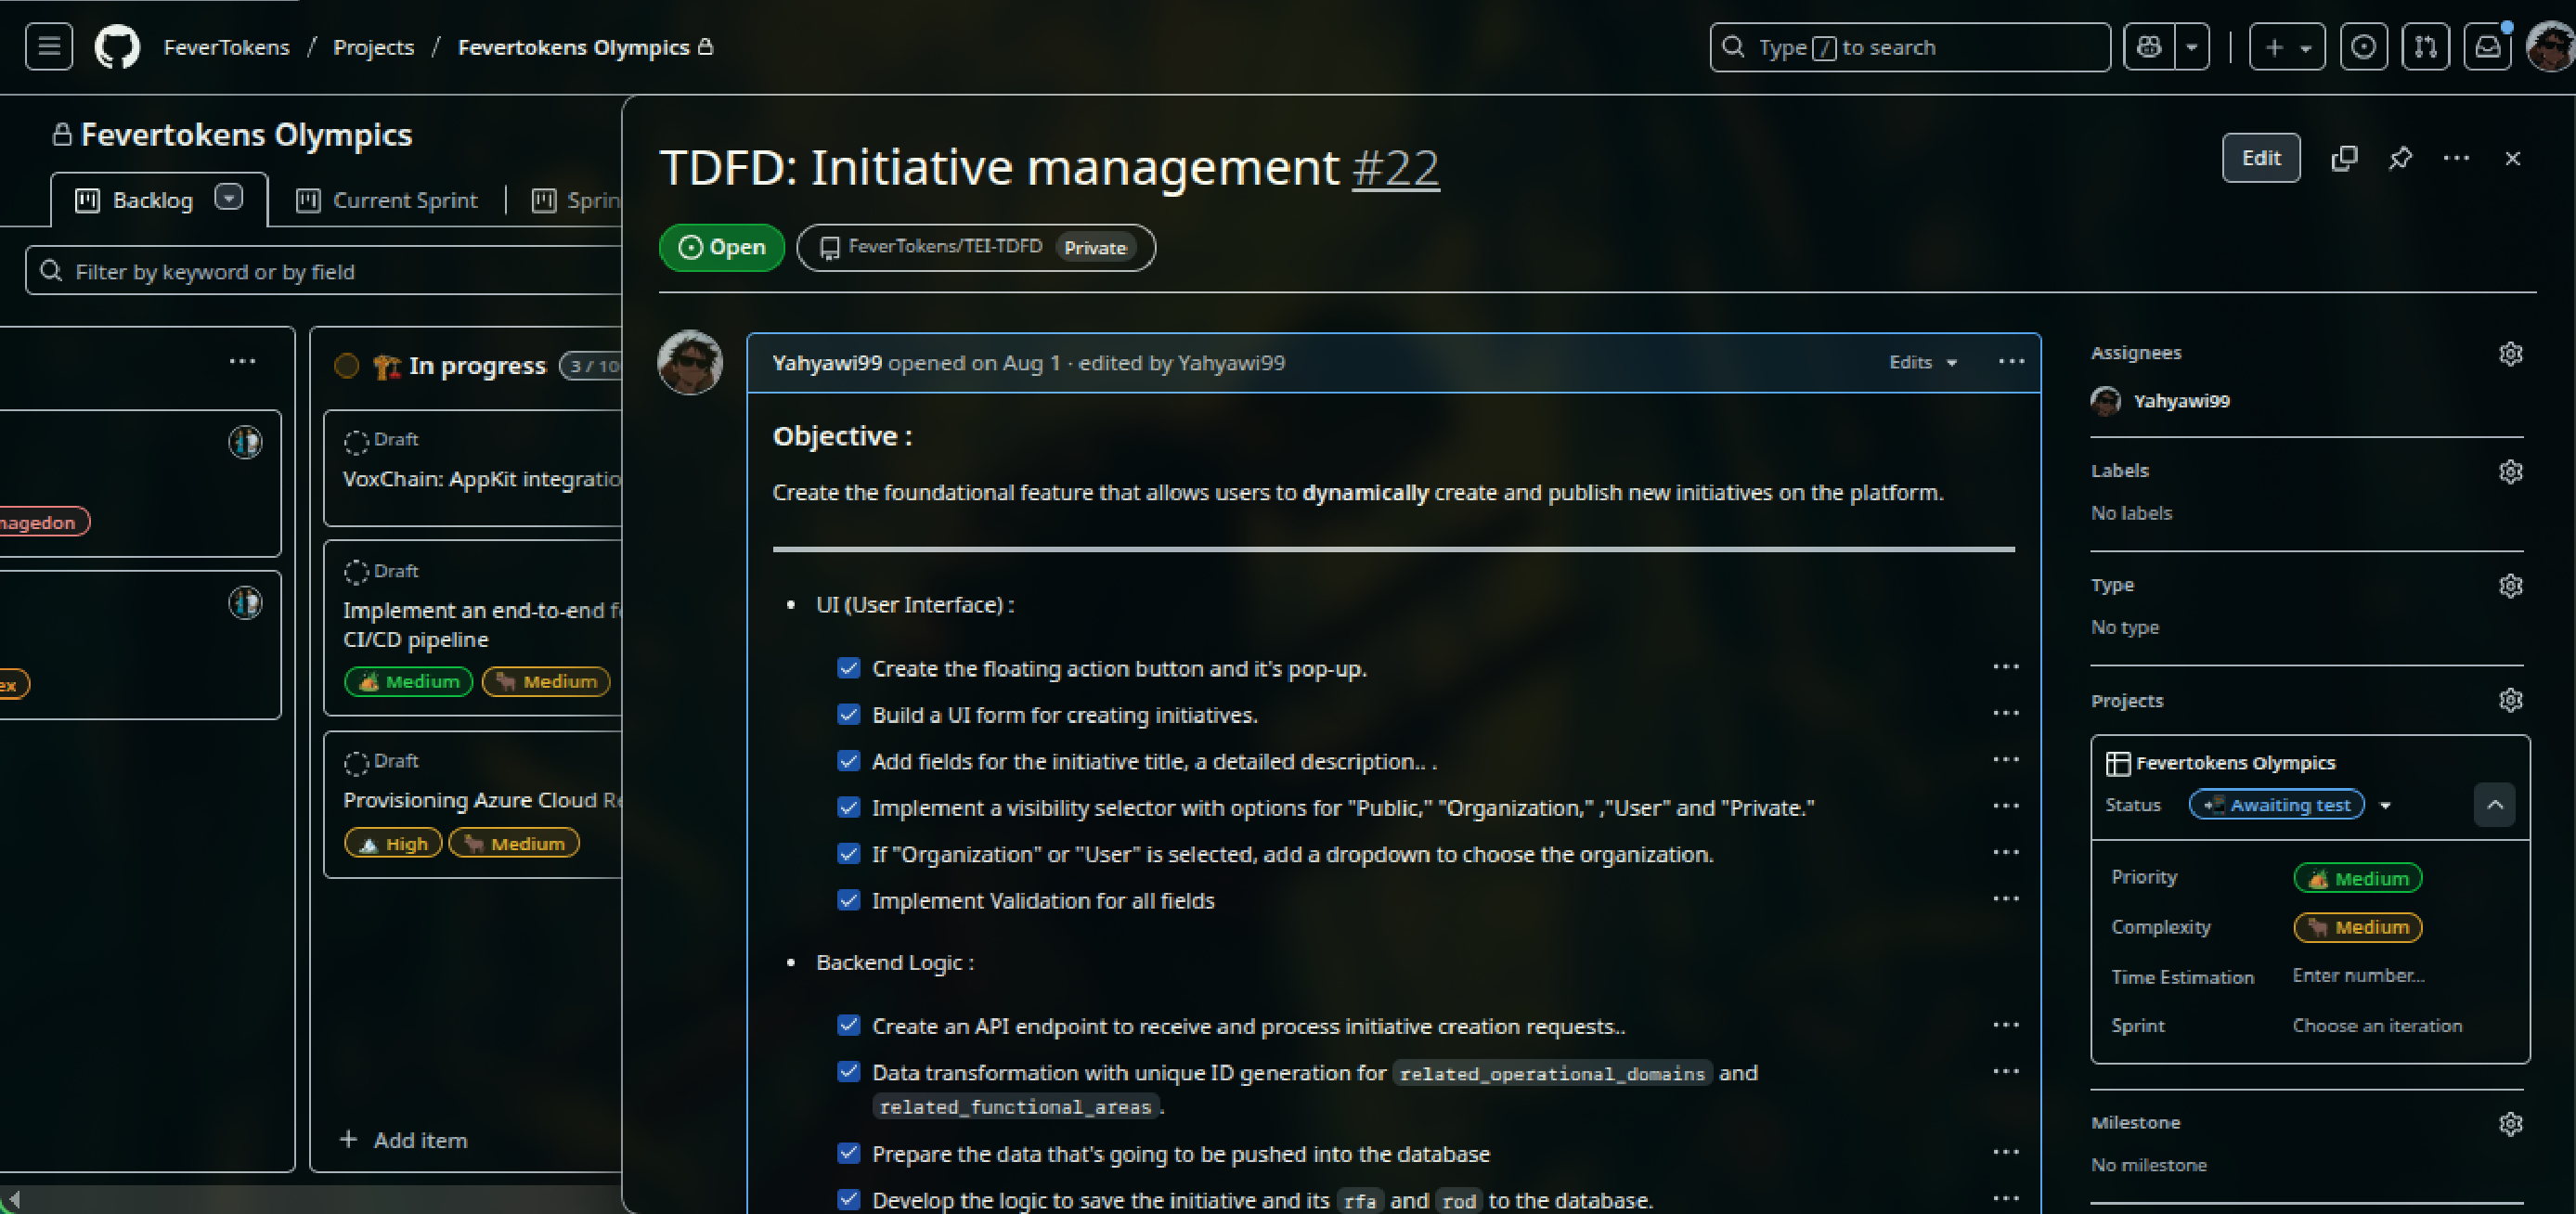
\includegraphics[width=0.7\textwidth]{figures/task.pdf}
    \caption{Exemple de tâche créée sur GitHub Projects}
    \label{fig:tache}
\end{figure}
\vskip.25cm
Le travail s'effectuait à distance avec des réunions quotidiennes (\textit{daily stand-ups}). Chaque stagiaire présentait brièvement les tâches réalisées la veille et celles planifiées pour la journée.\\[1mm]
Lorsqu'aucune tâche n'était attribuée, il fallait solliciter un nouveau travail auprès des superviseurs, garantissant ainsi une progression continue. Le suivi des tâches se faisait via \textbf{GitHub Projects}, ce qui permettait aux superviseurs de suivre l'avancement de chaque mission et de maintenir l'équipe synchronisée.\\[1mm]
En parallèle, chaque stagiaire devait préparer et présenter régulièrement un sujet spécifique attribué par l'un des superviseurs. Ces présentations n'étaient pas liées aux tâches quotidiennes mais servaient à approfondir nos connaissances sur des technologies ou concepts pertinents, tout en développant nos compétences en communication et présentation technique.\\

% ======= Technologies et outils utilisés =======
\section{Technologies et outils utilisés}
\leftskip.75cm
\subsection{Next.js}
\vskip.5cm
\begin{figure}[H]
    \centering
    
\includegraphics[width=0.6\textwidth]{figures/nextjs.pdf}
    \caption{Logo de Next.js}
    \label{fig:nextjs}
\end{figure}
\vskip1cm
Next.js m'a permis de développer des applications Web modernes en React avec un rendu côté serveur performant. L'utilisation de Next.js m'a aidé à comprendre l'organisation d'un projet full-stack, la gestion des routes, et l'optimisation des performances.\\

\subsection{TypeScript}
\begin{figure}[H]
    \centering
    
\includegraphics[width=0.6\textwidth]{figures/ts.pdf}
    \caption{Logo de TypeScript}
    \label{fig:typescript}
\end{figure}
\vskip.25cm
TypeScript a renforcé la qualité de mon code en ajoutant un typage strict, réduisant les erreurs à l'exécution. J'ai appris à structurer le code de manière claire et à anticiper les bugs grâce à la vérification statique des types.\\

\subsection{TailwindCSS}
\begin{figure}[H]
    \centering
    
\includegraphics[width=0.6\textwidth]{figures/tailwindcss.pdf}
    \caption{Logo de TailwindCSS}
    \label{fig:tailwind}
\end{figure}
L'utilisation de TailwindCSS a simplifié la création de styles cohérents et réactifs. Cela m'a permis de concevoir rapidement des interfaces utilisateur élégantes tout en respectant les standards de l'équipe\\

\subsection{PNPM}
\begin{figure}[H]
    \centering
    
\includegraphics[width=0.6\textwidth]{figures/pnpm.pdf}
    \caption{Logo de PNPM}
    \label{fig:pnpm}
\end{figure}
PNPM, le gestionnaire de paquets, a facilité la gestion des dépendances dans le monorepo.\\ J'ai appris à gérer plusieurs projets interconnectés de manière efficace et à maintenir la cohérence des versions.\\

\subsection{Base de données et ORM : MongoDB, Supabase, Prisma, Drizzle}
\vskip.5cm
\begin{figure}[H]
    \centering
    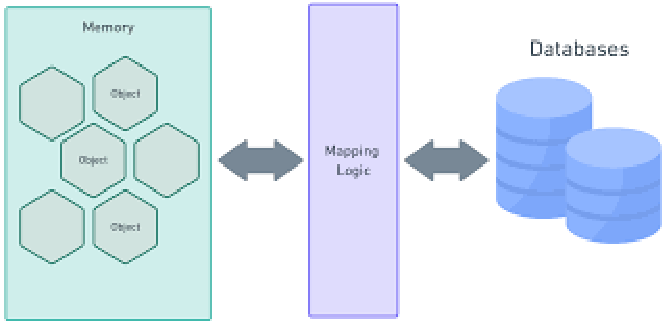
\includegraphics[width=0.6\textwidth]{figures/database.pdf}
    \caption{Bases de données et ORM}
    \label{fig:database}
\end{figure}
\vskip.25cm
Ces outils m'ont permis de concevoir et manipuler des bases de données complexes. J'ai appris à modéliser les données, à intégrer la base dans le projet, et à interagir efficacement avec l'ORM pour assurer la cohérence et la performance des requêtes.\\

\subsection{Better Auth}
\vskip.5cm
\begin{figure}[H]
    \centering
    
\includegraphics[width=0.6\textwidth]{figures/betterauth.pdf}
    \caption{Logo de Better Auth}
    \label{fig:betterauth}
\end{figure}
\vskip.25cm
Better Auth m'a permis de gérer l'authentification des utilisateurs de manière sécurisée et pratique. J'ai appris à implémenter l'inscription, la connexion, la gestion des sessions et la gestion des organisations grâce au plugin \textit{organization}.\\


\subsection{IA et assistants : LLMs, GitHub Copilot}
\vskip.5cm
\begin{figure}[H]
    \centering
    
\includegraphics[width=0.6\textwidth]{figures/AI.pdf}
    \caption{AI}
    \label{fig:copilot}
\end{figure}
\vskip.25cm
Ces outils m'ont assisté dans la génération de code, la conservation de temps et l'apprentissage rapide de nouvelles technologies. J'ai utilisé les \textbf{LLMs} pour créer des scripts et des composants de manière efficace, ce qui m'a permis de gagner du temps sur des tâches répétitives et de me concentrer sur l'apprentissage des bonnes pratiques. \textbf{Copilot} a également été utilisé pour améliorer la productivité et la qualité du code, tout en servant d'outil pédagogique pour découvrir de nouvelles méthodes de développement.\\

\subsection{Git, GitHub et VS Code}
\vskip-.6cm
\begin{figure}[H]
    \centering
    
\includegraphics[width=0.5\textwidth]{figures/github.pdf}
    \caption{Git-GitHub et VS Code}
    \label{fig:github}
\end{figure}
Git et GitHub ont été essentiels pour le versioning et la collaboration. VS Code a servi de plateforme principale de développement, permettant de travailler efficacement en équipe et de gérer le code source de manière structurée.\\

\subsection{Structure du monorepo et organisation des packages}
\vskip.5cm
\begin{figure}[H]
    \centering
    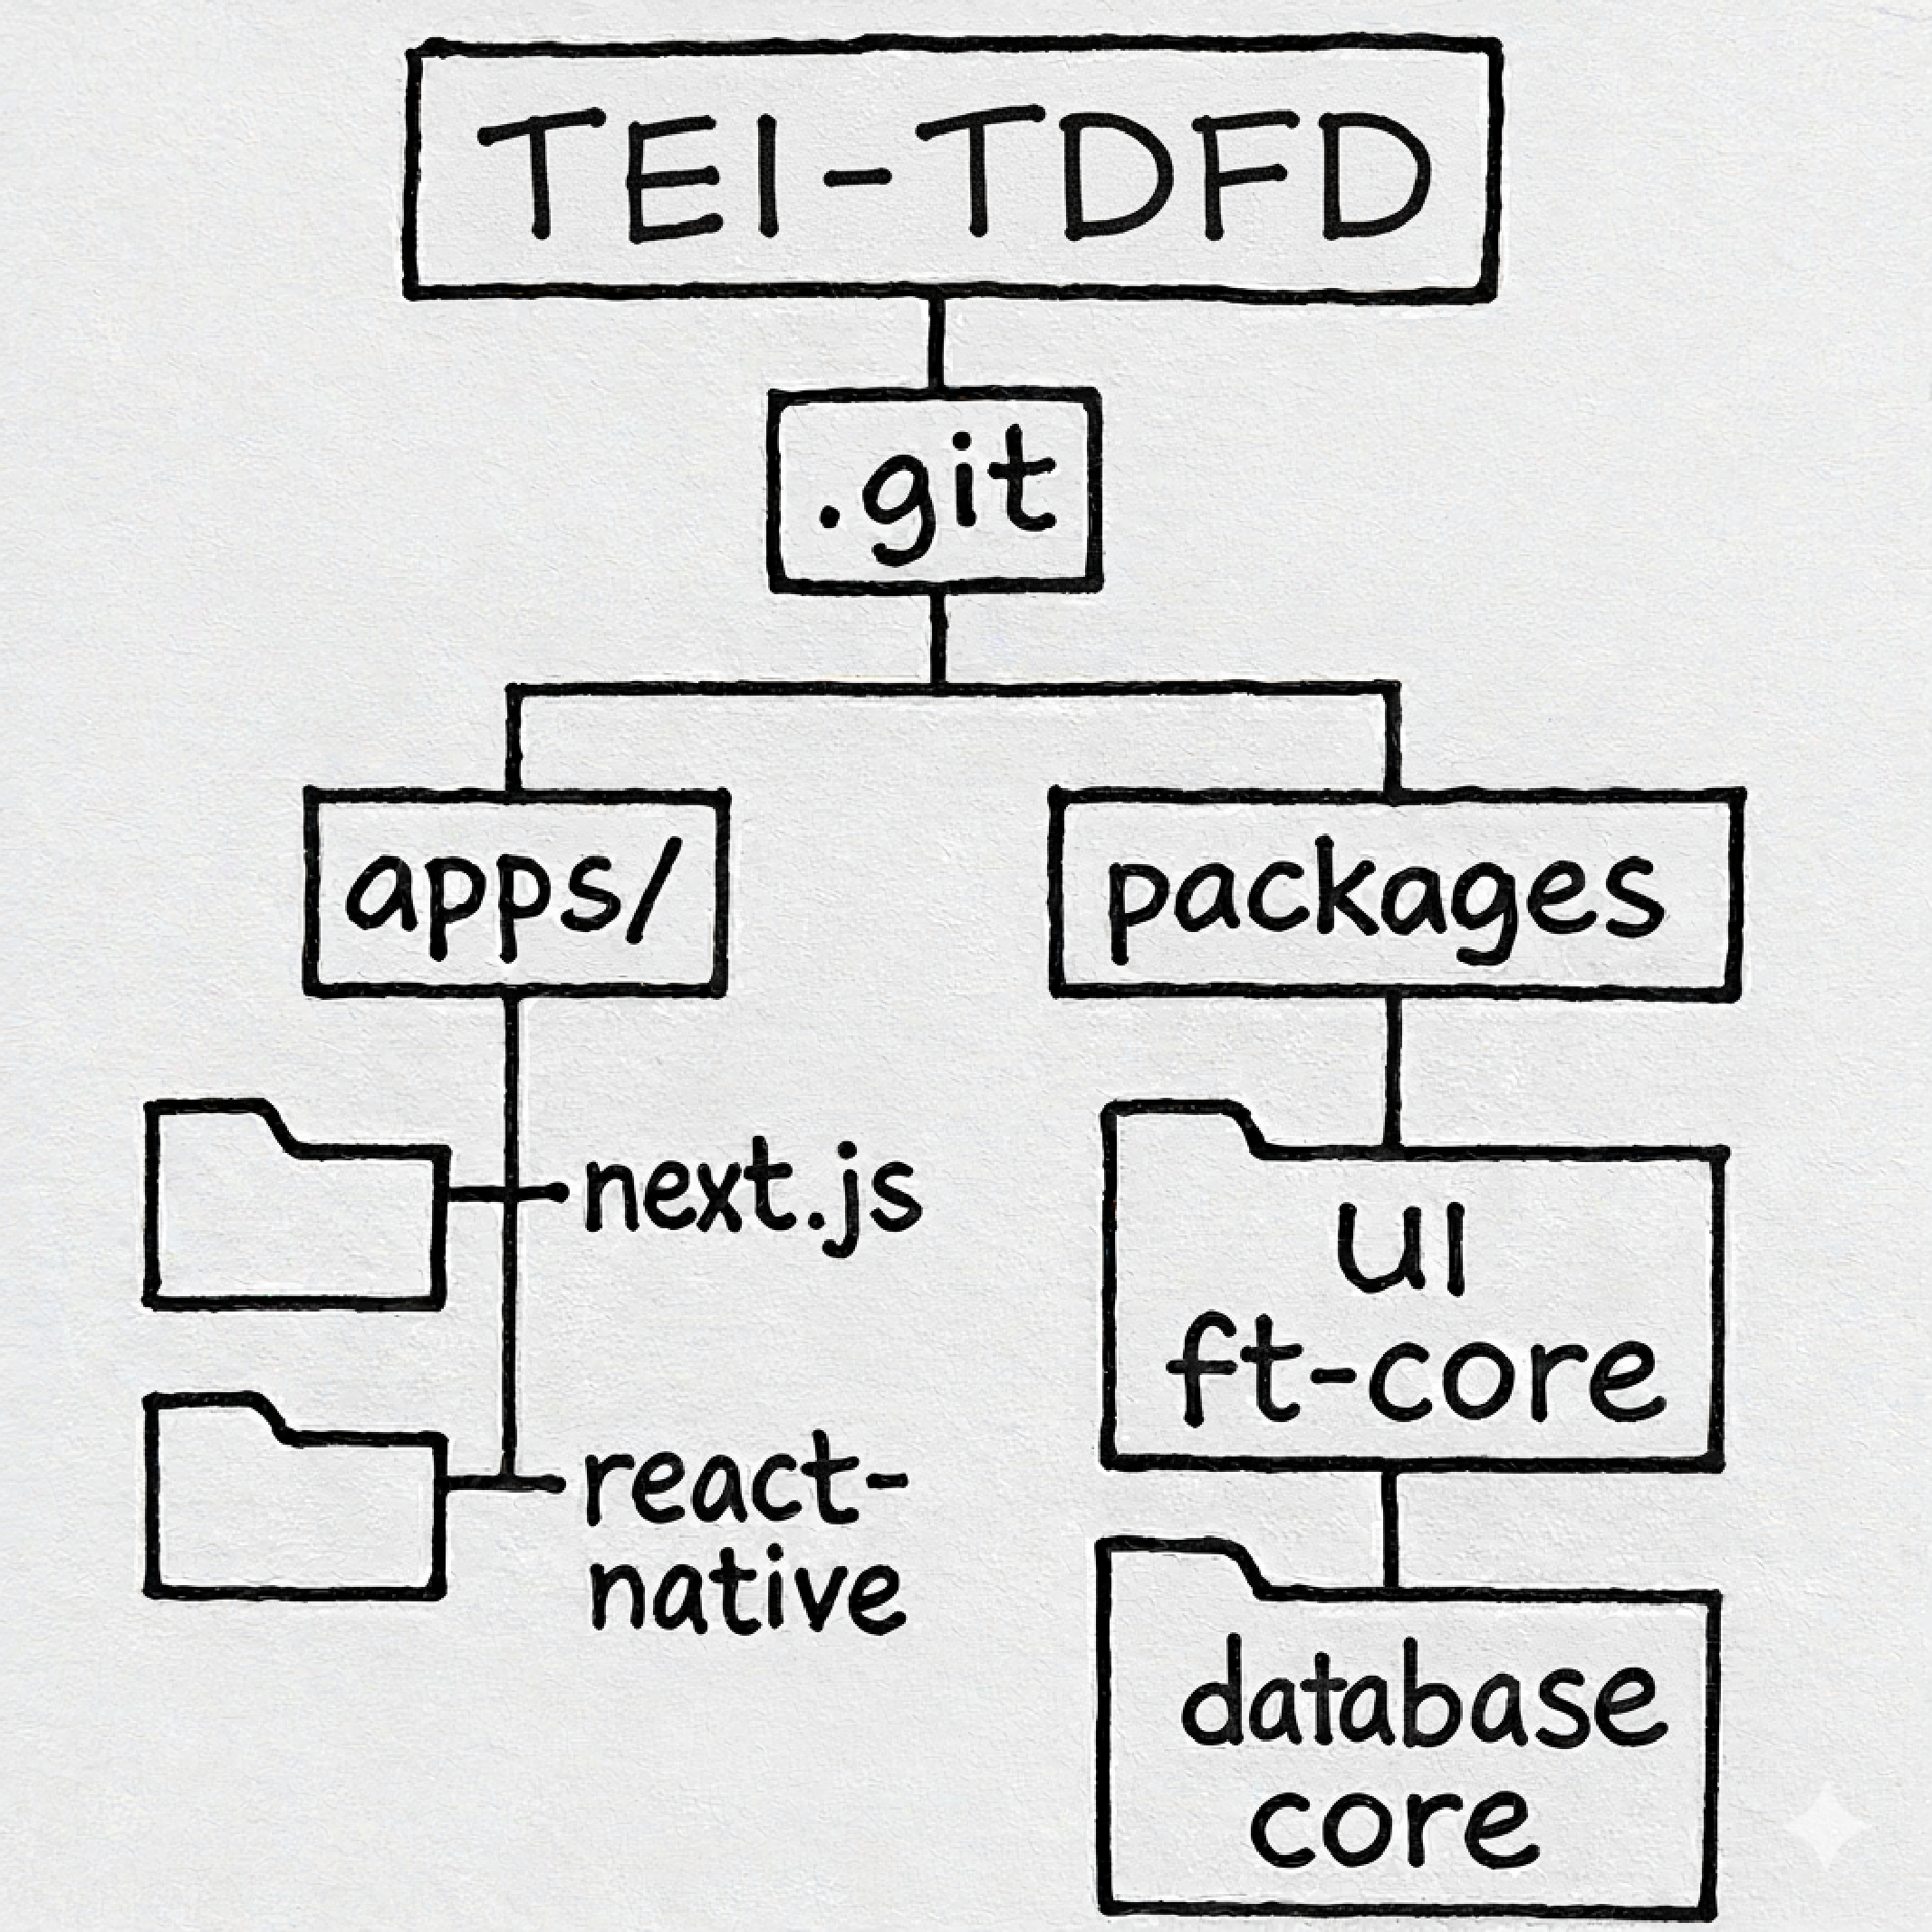
\includegraphics[width=0.4\textwidth]{figures/monorepo.pdf}
    \caption{Exemple de structure monorepo utilisée chez FeverTokens}
    \label{fig:monorepo}
\end{figure}
\vskip.25cm
Le projet était organisé en \textbf{monorepo}, regroupant plusieurs packages interconnectés dans un seul dépôt. Cette approche m'a permis de comprendre comment structurer un projet complexe tout en maintenant la cohérence entre les différents modules. J'ai appris à gérer les dépendances internes, à réutiliser du code entre packages, et à orchestrer le déploiement de plusieurs services interconnectés. Le monorepo facilite également le versioning et la collaboration, car chaque modification est centralisée et visible par tous les membres de l'équipe, ce qui a amélioré ma compréhension de l'intégration continue et de la gestion de projet full-stack.\\

\leftskip0cm

% ======= Conclusion =======
\section{Conclusion}
L'utilisation combinée de ces technologies et outils a permis un apprentissage pratique approfondi, le développement de compétences techniques en full-stack, et une collaboration efficace au sein de l'équipe.\\[1mm]
Chaque outil a contribué à améliorer la qualité du code, l'organisation du travail et la coordination entre les membres de l'équipe.
